\chapter{Literature Review}

This chapter reviews the reseach papers, articles, books and other relevant form of researches used in the design of the NPSC. It has been divided into the sectioned below:
\begin{itemize}
\item The human sleep-wake cycle
\item Previous attempts
\item Hardware modules and PCB design requirements
\item Communication protocols
\item Programming Languages
\item Software Tools and Libraries
\end{itemize}

%%%%%%%%%%%%%%%%%%%%%%%%%%%%%%%%%%%%%%%%%%%%%%%%%%%%%%%%%%%%%%%%%%%%%%%%%%%%%%%%%%%%
% SECTION: The human sleep-wake cycle
%%%%%%%%%%%%%%%%%%%%%%%%%%%%%%%%%%%%%%%%%%%%%%%%%%%%%%%%%%%%%%%%%%%%%%%%%%%%%%%%%%%%
\section{The human sleep-wake cycle}
\subsection{The circadian rhythm}

Many of our seasonal behaviour are synchronised to the environment by \textbf{biological clocks} responsible for the creation of circadian rhythms. Biological clocks which are composed of protein that act reciprocally on the body's cells are the natural timing device found in many organs. The discovery of the genes from these biological clocks responsible for the control of the circadian rhythms was made by three scientists Jeffrey  C.  Hall,  Michael  Rosbash  and Michael W. Young winners of the Nobel Prize in Physiology or Medicine \cite{sc2017}. Their discovery made in the 1980s led to advanced research on the role of the circadian rhythms.\\
Circadian rhythms are biological rhythms which follow the same pattern in absence of external cues (endegenous), are influenced by the presence of external stimuli (entertainable), oxillating every 24h over a range of phisiological temperatures. In the presence of external stimuli -also known as \textit{zeitgebers}-, circadian rhythms synchronise their periodicity with these external stimuli. The zeitgebers of the circadian are the daily variation of the temperature and the dark/light cycle of the day.\\
Circadian rhythms have an endegenous and an exogenous components. Human placed in isolation without knowledge of the time continued exhibiting a circadian rhythm with their pacemakers notably the melatonin secretion, sleep-wake cycle, body temperature \cite{in1996}. These results proove the endegenous component of the circadian rhythms. A similar study shows that when people are exposed to light at night time, a shift in their pacemakers \cite{ea2004} which is an evidence of the exogenous component of circadian rhythms.\\
The exogenous components of the circadian rhythms have the ability affect positively and begatively our natural endogenous cycle. With light being what we are mostly daily exposed to, what is the influence of light on the circadian thythms? 

\subsection{Internal circadian rhythms influenced by light}
Melatonin is the hormone produced by the pineal gland in the suprachiasmatic nuclei (SCN) which has a soporific effect and the ability to entertain the sleep-wake cycle. While melatonin itself is not the cause of a person sleeping, it however creates changes in a person's body that affect their sleepiness. \\
The pineal gland responsible for the secretion of the melatonin hormone is under the influence of one of the biological clocks, the master clock located in the SCN. The SCN receives visual information from the retinal-hypothalamic tract which entrains the SCN according to the photoperiod \cite{lig1994}. The SCN in turn activate a gene in the pineal cell (CREM) which produce a protein (ICER) needed for the production of melatonin. As a result, the secretion of pineal hormone melatonin follow the light/dark cycle with its  secretion being high during the day and low during the night.  

\subsection{Quantitative and qualitative characteristics of light on melatonin production}
Many researches have been done to understand the impact of light on the circadian rhythms expecially the sleep-wake cycle. \\
Kathleen \textit{et al.} in their paper \textit{Blue light from light-emitting diodes elicits a dose-dependent suppression of melatonin in humans}\cite{bl2010}, provide details information on their finding of  the effect of light on humans subject. Subjects used for the expirements were 5 males and 3 females with an mean of $23.9\pm0.5$ years, with each subject demonstrating normal color vision. The lighting requirment was blue light of $\lambda_{max} = 469nm \pm 1nm $ with $\frac{1}{2}$ peak bandwidth$ = 26nm$ and a typical viewing distance of $35cm$. The subjects were blindfolded from midnight to 2AM. From thereon, they were exposed to 90 min of blue light exposure  followed by another dark exposure. Blood sample from the subject were taken from 2AM at 30 min interval.From their experiment, they concluded that:
\begin{itemize}
\item \textbf{Blue LED light has an increased melatonin supression following an increase in exposure irradiance}
\item \textbf{Blue LED light may have stronger suppressing effect than 4000K white fluorescent light.}
\end{itemize}
A similar study was previously made by George C. Brainard \textit{et al.} \cite{ac2001} used 72 healthy human subjects, with normal color vision. The subjects composed of 37 females, 35 males, aged between 18 and 30 years (mean age of $24.5 \pm 0.3$ years), came from different ethnic (african, african americans, caucasians, asian, hispanic). The melatonin suppression action spectrum was formed using eight different wavelengths between $440nm$ and $600nm$ \textit{(440, 460, 480, 505, 530, 555, 575, 600)}. Using the same procedure as mentioned in the previous experiment, blood samples were taken at 30 min interval after 2AM. The results of their research published in their paper \textit{Action Spectrum for Melatonin Regulation in Humans: Evidence for a Novel Circadian Photoreceptor} the following conclusion:
\begin{itemize}
\item \textbf{Light irradiance greater or equal to $3.1 \mu W/cm^{2}$ evoke a significant melatonin supression}
\item \textbf{Smaller wavelenght monochromatic light have a greater change in \textit{Plasma Melatonin as Percent Change Control-Adjusted} for a fixed value of \textit{Photon density}} (\cite{ac2001} pp. 4-5).
\end{itemize}   

\subsection{Impact of light on human behaviour and sleep-wake cycle}
Among the Zeitgebers of the circadian rhythms, light being the major Zeitgebers has important effect on the human sleep-wake cycle. Christian \textit{et al.}\cite{cir2014} shown that subjective sleepiness and core body temperature opposes each other (\cite{cir2014}, pp. 12, fig. 2.1) when there is no phase lag or lead between the endogenous circadian rhythm and the sleep-wake cycle. The human normal sleep-wake cycle is comprised of 8h of sleep and 16h of wakefulness \cite{is1995}. This cycle is naturally affected by the human activities but is highly inflenced by light exposure. The study shows that office workers with bright blue office light have a better sleep-wake cycle than those with dim and warm office light. Furthermore, it shows that light exposure of sufficient intensity at night can reduce the secretion of melatonin with alerting response starting within the first 20mn. With the recent advance in LED technologies, human are no longer following the natural light/dark cycle causing numerous sleep disorders. 

  
%%%%%%%%%%%%%%%%%%%%%%%%%%%%%%%%%%%%%%%%%%%%%%%%%%%%%%%%%%%%%%%%%%%%%%%%%%%%%%%%%%%%
% SECTION: LEDs technologies
%%%%%%%%%%%%%%%%%%%%%%%%%%%%%%%%%%%%%%%%%%%%%%%%%%%%%%%%%%%%%%%%%%%%%%%%%%%%%%%%%%%%
\section{Lighting technologies}

\subsection{Artificial and natural light}
The sun's electromagnetic rediation has a broad light spectrum ranging from  $100nm$ to $1mm$. After being filtered through the earth atmosphere, only certain portions of the spectrum are kept with the visible light spectrum having the maximum irradiance. LED technologies are able to produce more or less the same wavelenght as the sunlight but with much less irradiance. 

\subsection{Light treatment of sleep disorder}
With the discovery of the effect of light on the sleep-wake cycle, electronic devices producing specific light requirment have been used in treating patient with sleep discorder. Advanced sleep phase disorder (ASPD) have been treated using a therapeutic approach involving chronotherapy and timed light exposure \cite{th2010}. The same concept has been used to create a home bed lamp or alarm clock facilitating the regualtion of the slepp-wake cycle. \textbf{GE Sol} and \textbf{Philips}\textit{(which is actively involved in sleep-wake cycle treatement)} have created devices able to ``influence'' the human sleep-wakr cycle.

\subsubsection{C by GE Sol}
\textit{C} shown in \cref{fig:c} is a ``all-in-one smart light'' \cite{gesol} which has Amazon intelligent personal assistant Alexa built in. C has a various range of colours which are manually selected based on the user preference. It is capable of communicating wiht GE sol devices and smartphones inserting it among the user's network of devices. Despite its high technology features and its elegant design, C remains just a bed lamp as it is not clinically proven to be helpful in regulating the user's sleep-wake cycle.
\begin{figure}[ht]
\centering
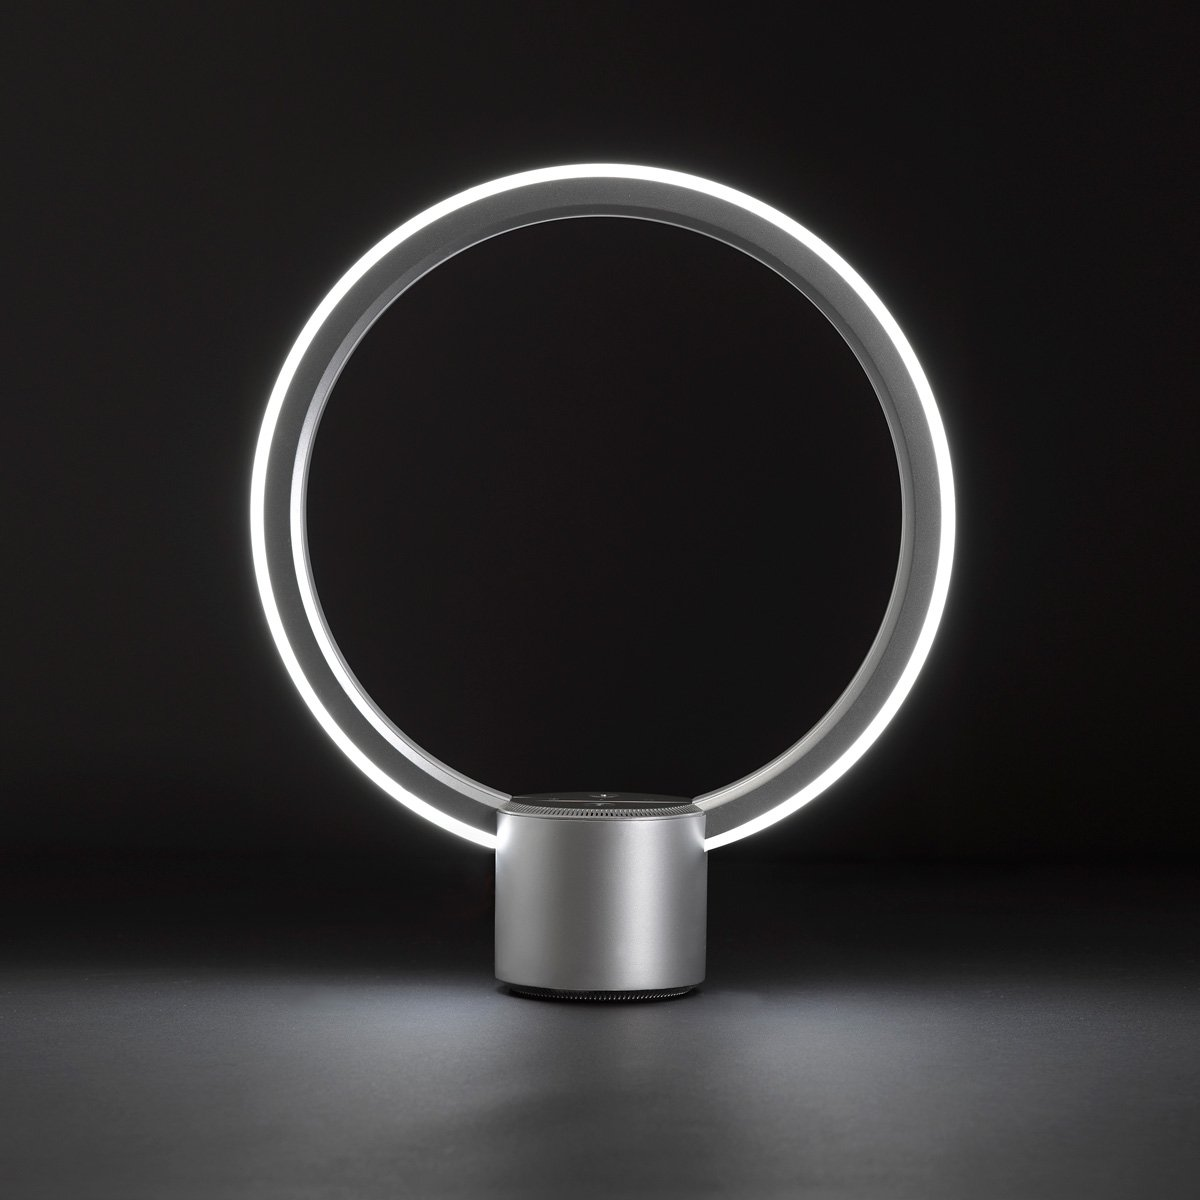
\includegraphics[scale=0.2]{sol1.jpg}
\caption{C by GE Sol, an intelligent lamp bed using Amazon Alextra.}
\label{fig:c}
\end{figure}

\subsubsection{Philips wake-up lamps}
Philips has created a broad range of wake-up lamps designed to impact the sleep-wake cycle of the users. \Cref{fig:philips1,fig:philips2} are examples of the recent versions of Philips' clocks able to simulate sunrise and sunset which last from 20 to 40 mn. These simulations vary the colour of the light following the sun's natural sunrise colour and end with a selected channel or prefered user's music. These Sleep and Wake-up lights are the only wake-up lamp clinically proven to work as claimed by Philips\cite{philips}. 

\begin{figure}[ht]
\centering
\begin{minipage}[b]{0.45\textwidth}
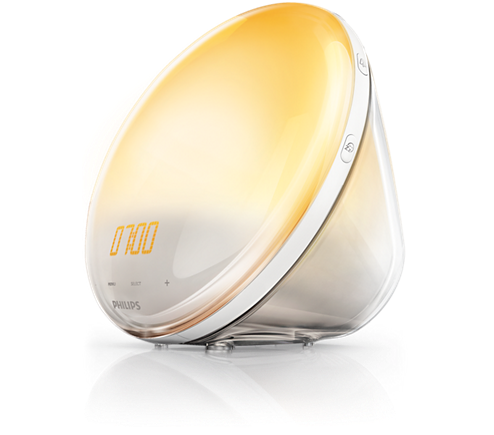
\includegraphics[scale=0.4]{philips1.png}
\subcaption[first caption.]{HF3531/60, coloured sunrise\\ simulation, 7 natural sounds, Tap\\ snooze and reading lamp, midnight\\ light function}
\label{fig:philips1}
\end{minipage}
\begin{minipage}[b]{0.45\textwidth}
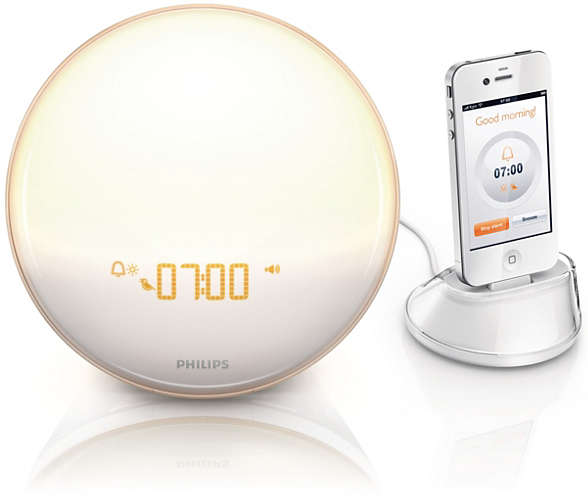
\includegraphics[scale=0.35]{philips2.jpeg}
\subcaption[second caption.]{HF3551/60, coloured sunrise simulation, 7 natural sounds, Tap snooze and reading lamp, midnight light function, Operated by iPhone App}
\label{fig:philips2}
\end{minipage}
\caption{Wake-up light by Philips}
\label{philips}
\end{figure}



%%%%%%%%%%%%%%%%%%%%%%%%%%%%%%%%%%%%%%%%%%%%%%%%%%%%%%%%%%%%%%%%%%%%%%%%%%%%%%%%%%%%
% SECTION: Hardware modules 
%%%%%%%%%%%%%%%%%%%%%%%%%%%%%%%%%%%%%%%%%%%%%%%%%%%%%%%%%%%%%%%%%%%%%%%%%%%%%%%%%%%%
\section{Hardware modules}

\subsection{Processors and microcontrollers}
A microcontroller is a computer, it contains a central processing unit (CPU), it has some random access menory (RAM), it has input and output peripherals. However, a microcontroller is way smaller, cheaper, use less electrical power, and has less processing capabilities than a computer making it the preference for tasks specific electronic design \cite{ho2000}.\\
Numerous microcontrollers were analysed for this project. Each manufacturer provide various range of microcontroller suitable for different application. In order to reduce the complexity of finding the \textit{perfect} microcontroller for the NPSC, the selection was based on the following characteristics:
\begin{itemize}
\item \textbf{Size of the FLASH:} How many lines of code can be loaded to the microcontroller?
\item \textbf{Cost}
\item \textbf{Clock speed}
\item \textbf{Community:} Does the manufacturer have a large community of developers?
\item \textbf{Bit precision:} Are we aiming at 8, 16, or 32 bits precision? 
\item \textbf{Familiarity:} How familliar are we with the microcontroller (time is a constraint)?
\item \textbf{Number of pins:} How familliar are we with the microcontroller (time is a constraint)?\
\item \textbf{Extra features:} What are then built-in functionalities (wifi module, bluetooth)?
\end{itemize}

\Cref{table:micro} provides the difference between the microcontrollers selected, this table was use in making the final decision of the microcontroller selection.
\begin{table}[h!]
\centering
\begin{tabular}{cp{5em}p{8em}p{5em}c}
\hline
\hline
\multirow{2}{*}{Characteristics}  & \multicolumn{4}{c}{Microcontrollers} \\  
 & \textbf{Arduino Due} & \textbf{Intel Edison} & \textbf{Raspberry Pi Zero} & \textbf{STM32F407VGT6} \\
\hline
\textbf{Clock speed} & 84MHz &  dual-core, dual-threaded 500 MHz CPU & 1GHz single core & 168 MHz\\
\textbf{Bit precision} & 32 & 32 & 32 & 32 \\
\textbf{FLASH} & 512KB & 4GB & MicroSDHC & 1MB \\
\textbf{Pins} & 54 & 40 & 40 & 82\\
\textbf{Cost} & R549.25 & R687.87 & R79.8 & R175.45\\
\hline
\hline
\end{tabular}
\caption{Comparison between specifications of the Arduino Due \cite{arduino}, the Intel Edison \cite{intel}, the Raspverry Pi Zero \cite{raspberry}, and the STM32F407VGT6\cite{stm}}
\label{table:micro}
\end{table}

%\subsection{LEDs}
%We have come a long way since the first commercialisable light bulb was patented Thomas Edison. Nowadays the generic light buld has been replaced by more efficient lighting technologies. In order to understand  the differences between these new technologies, the quantitative and qualitative parameters of light must be understood.
%
%\subsubsection{Explanation of the light parameters}
%\begin{itemize}
%\item \textbf{Colour Rendering Index (CRI):} Ranging between 1 and 100, CRI is a measure of the ability of a light source to render excatly all the frequency of its colour spectrum compared to a natural light source. The higher the rating, the more accurate is the rendering.   
%\item \textbf{Colour Temperature (CT):} Simply put, it is the description of the characteristic of light,classifying the light as either warm or cool and measured in Kelvin.  
%\item \textbf{Luminous intensity:} Amount of light (more specifically the wavelength weighted power) emmitted   in a specific direction per unit of solid angle.
%\item \textbf{Luminous flux:} The measure of the amount of light emitted by a source, or received by a surface.
%\item \textbf{Luminance:} The measure of the luminance intensity in a given direction per unit area. 
%\item \textbf{Illuminance:} The luminous flux arriving at a particular point of a surface from all direction.
%\item \textbf{Luminous efficacy:} The ratio of light output to electrical power
%\end{itemize}
%The mathematical expression of some of these characteristics is tabulated in \cref{table:light} .
%\begin{table}[h!]
%\centering
%\begin{tabular}{ccc}
%\hline
%\hline
%\textbf{Characteristics} & \textbf{Formula} & \textbf{Units} \\
%\hline
%Luminous flux & F & Lumen (lm) \\
%Luminous intensity & $I=\frac{F}{\omega}$ & Candela (cd) \\
%Luminance & L & candela per square meter ($\frac{cd}{m^2}$) \\
%Illuminance & $E=\frac{F}{A}$ & Lux (lx) \\
%\hline
%\hline
%\end{tabular}
%\caption{Mathematical expressions of the light parameters}
%\label{table:light} 
%\end{table}
%\subsubsection{Introducing LEDs}
%* debuts\\
%* efficiency \\
%* newer tech (colour range, wifi, ...) \\
%* popularity \\

\subsection{LEDs}
types of LEDs technology and introduction of the neopixels
\subsection{Storage}
Storages are important in the development of embedded solutions. The \textbf{Electrical Erasable Programmable Read-Only Memory} (EEPROM) is a non-volatile memory capable of keeping its data after being powered off. Its design was based on the \textbf{Erasable Programmable Read-Only Memory} (EPROM) which required exposure to UV light for erasing its memory. There are two types of EEPROMs, serial and parallel EEPROMs. In a study made by Microship on the difference between serial and parallel EEPROM of 16KB, Tom Tyson from the Memory Product Divisions concluded that the serial EEPROM is \textit{the best option for embedded solutions requiring a small EEPROM footprint, low current and low operating voltage, the ability and ease to programme a byte at a time, and the best price performance non-volatile memory solution available}\cite{serialvsparallel} (pp. 4).


\subsection{Wireless technology}
Different types of wireless technologies allow devices to commnunicate to each other wirelessly. The Institute of Electrical and Electronics Engineers (IEEE) has grouped them in the 802.15 technologies. Among these are the well known Wifi, the cellular machine to machine (M2M), the mesh network using \textbf{ZigBee}, \textbf{Z-wave} \ldots . Bluettoth is the wireless technology of interest in this project. Bluetooth invented in 1994 is an open standard for short range wireless communication. While being low cost, it is subject to limitations namely its short range of operation being arroung 10m \footnote{Can be increased by increasing the transmission power} and its low transmission rate (780kb/s). 

\subsection{Touch screen}
A touch-screen device can locate the position of a point of contact on its screen. The idea of a using  contact presure of a object in application was initially from Hugh Le Caine with his Electronic Slackbut capable of change the volume of musical notes based on the amount of pressure applied to the keys. Later in 1969, E. A. Johnson created two major touch-screen technologies using a resistive and a capacitive approach. \\
A resistive touch-screen is made out of many layers among which two are composed of indium-tin oxide (ITO) which is highly resistive and transparent. By applying pressure on one of the layer, the layers come in contact creating a signal that is used to find the location of the point of contact. A capacitive touch-screen make use of the conductivity of the object in contact with the screen to affect the electrostatic field between the ITO layers. \\
Resistive touch-screen are less complex than capacitive touch-screen, thus cheaper. Moreover, because it relies on pressure, any object whether conductive or not can be used on the screen. One the other side, resistive touch-screen do not support multi-touch and have poor contrast becaused of the extra layer used to protect the ITO layers.
\begin{figure}[ht]
\centering
\begin{minipage}[b]{0.45\textwidth}
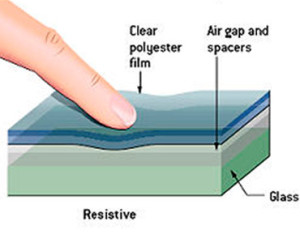
\includegraphics[scale=0.4]{resistiveTouch.jpg}
\subcaption[first caption.]{Resistive touch-screen technology\cite{resistivetouch}.}
\label{fig:philips1}
\end{minipage}
\begin{minipage}[b]{0.45\textwidth}
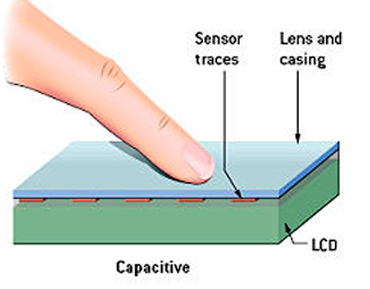
\includegraphics[scale=0.35]{capacitiveTouch.jpg}
\subcaption[second caption.]{Resistive touch-screen technology \cite{capacitivetouch}.}
\label{fig:philips2}
\end{minipage}
\caption{Touch-screen technologies}
\label{philips}
\end{figure}    


%%%%%%%%%%%%%%%%%%%%%%%%%%%%%%%%%%%%%%%%%%%%%%%%%%%%%%%%%%%%%%%%%%%%%%%%%%%%%%%%%%%%
% SECTION: Communication protocols
%%%%%%%%%%%%%%%%%%%%%%%%%%%%%%%%%%%%%%%%%%%%%%%%%%%%%%%%%%%%%%%%%%%%%%%%%%%%%%%%%%%%
\section{Communication protocols}
Communication protocols
\subsection{Serial Peripheral Interface (SPI) Bus}
SPI is a synchronous full duplex serial communication protocol used for short distance communication of electronic devices. With the protocol, one master can communicate to many slaves using a chip select pin (use to select the slave) but a slave can only talk to the master device. SPI uses 4 signals namely, the Master Out Slave In (MOSI), the Master In Slave Out (MISO), the clock (SCK), and the slave select or chip select (SS). Since SPI uses a clock, it does not require the configuration of a baud rate before communication. The main inconvenience with SPI is the number of pin require for a one to one communication, for every additional slave, the master must provide a SS pins which make SPI not the ideal protocol for communicating to multiple slaves devices \cite{spi}. 
\subsection{Universal asynchronous receiver-transmitter (UART)}
UART is a asynchronous full duplex communication protocol making use of two signals a transmit signal (TX) and a receive signal (RX). With UART, both devices need to agree on a baud-rate for communication, this rate define the number of bytes to be sent and received. The problem with UART is the complexity of the protocol required to ensure synchronous communication and correct transfer of information between device. Although theoretically UART baud-rate is infinite, it is practically limited to 230400 bits per seconds \cite{uart}.   
\subsection{Inter-Integrated Circuit (I2C)}
I2C is a serial protocol that allows communications fom multiple slaves to multiple masters. It takes a bit of both SPI and UART by being designed for short distance communication and requiring only two pins, namely the data line (SDA) and clock line (SCL). Its clock ranges from $100kHz$ to $400kHz$ and a bytes is sent at a time. Furthermore with the I2C protocol, each slave must have a unique address used by the master for communication \cite{i2c}.  
\subsection{Neopixels}
Each neopixel has a built-in IC controlling the LEDs' intensity based on the data receive. The neopixels use a single wire communication protocol. When connected in series, the neopixels form a daisy chain allowing the programmation of a serie of neopixels using one signal. \\
Each neopixel requires 24 Bytes (32 Bytes for RGBW LEDs), each bytes is an encoded bit using a Non-Return-to-Zero encoding. \Cref{fig:nrz} shows the encoding pulses used.  
\begin{figure}[ht]
\centering
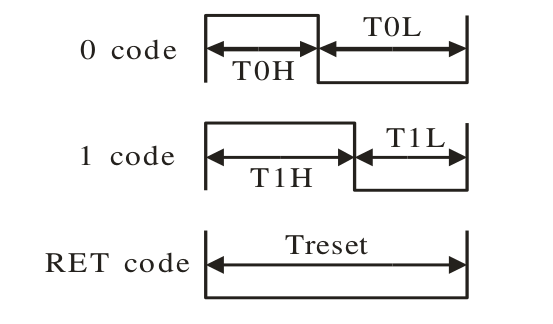
\includegraphics[scale=0.4]{nrz.png}
\caption{Non-return-to-zero encoding of a single bit in the neopixels programming protocol}
\label{fig:nrz}
\end{figure}
    
%%%%%%%%%%%%%%%%%%%%%%%%%%%%%%%%%%%%%%%%%%%%%%%%%%%%%%%%%%%%%%%%%%%%%%%%%%%%%%%%%%%%
% SECTION: PCB Board Design
%%%%%%%%%%%%%%%%%%%%%%%%%%%%%%%%%%%%%%%%%%%%%%%%%%%%%%%%%%%%%%%%%%%%%%%%%%%%%%%%%%%%
\section{PCB Board Design}
PCB Board Design
advice, best practices

%%%%%%%%%%%%%%%%%%%%%%%%%%%%%%%%%%%%%%%%%%%%%%%%%%%%%%%%%%%%%%%%%%%%%%%%%%%%%%%%%%%%
% SECTION: Software
%%%%%%%%%%%%%%%%%%%%%%%%%%%%%%%%%%%%%%%%%%%%%%%%%%%%%%%%%%%%%%%%%%%%%%%%%%%%%%%%%%%%
\section{Programming Languages}



%%%%%%%%%%%%%%%%%%%%%%%%%%%%%%%%%%%%%%%%%%%%%%%%%%%%%%%%%%%%%%%%%%%%%%%%%%%%%%%%%%%%
% SECTION: Software Tools and Libraries
%%%%%%%%%%%%%%%%%%%%%%%%%%%%%%%%%%%%%%%%%%%%%%%%%%%%%%%%%%%%%%%%%%%%%%%%%%%%%%%%%%%%
\section{Software Tools and Libraries}
Software Tools and Libraries 
\subsection{Toolchain}
\subsection{Nextion}
\subsection{Android Application}


A literature review forms the theoretical basis of your project. You need to read a large number of
journal papers, sections in books, technical reports etc. relevant to your work at the start of project.
This will give you a good idea of the field of research.

When writing your review start of with the general concepts and move to the more specific aspects
explaining the necessary theory as you go. This section is NOT a copy and paste from others work or a
rewrite-but-change-one-word section. I suggest you read all your material, and then put it down and
write this section, referring back to the work only when you need to check something.

See your PCS textbook for more details on how to write a literature review.


